%
%Не забыть:
%--------------------------------------
%Вставить колонтитулы, поменять название на титульнике



%--------------------------------------

\documentclass[a4paper, 12pt]{article} 

%--------------------------------------
%Russian-specific packages
%--------------------------------------
%\usepackage[warn]{mathtext}
\usepackage[T2A]{fontenc}
\usepackage[utf8]{inputenc}
\usepackage[english,russian]{babel}
\usepackage[intlimits]{amsmath}
\usepackage{esint}
%--------------------------------------
%Hyphenation rules
%--------------------------------------
\usepackage{hyphenat}
\hyphenation{ма-те-ма-ти-ка вос-ста-нав-ли-вать}
%--------------------------------------
%Packages
%--------------------------------------
\usepackage{amsmath}
\usepackage{amssymb}
\usepackage{amsfonts}
\usepackage{amsthm}
\usepackage{latexsym}
\usepackage{mathtools}
\usepackage{etoolbox}%Булевые операторы
\usepackage{extsizes}%Выставление произвольного шрифта в \documentclass
\usepackage{geometry}%Разметка листа
\usepackage{indentfirst}
\usepackage{wrapfig}%Создание обтекаемых текстом объектов
\usepackage{fancyhdr}%Создание колонтитулов
\usepackage{setspace}%Настройка интерлиньяжа
\usepackage{lastpage}%Вывод номера последней страницы в документе, \lastpage
\usepackage{soul}%Изменение параметров начертания
\usepackage{hyperref}%Две строчки с настройкой гиперссылок внутри получаеммого
\usepackage[usenames,dvipsnames,svgnames,table,rgb]{xcolor}% pdf-документа
\usepackage{multicol}%Позволяет писать текст в несколько колонок
\usepackage{cite}%Работа с библиографией
\usepackage{subfigure}% Человеческая вставка нескольких картинок
\usepackage{tikz}%Рисование рисунков
\usepackage{float}% Возможность ставить H в положениях картинки
% Для картинок Моти
\usepackage{misccorr}
\usepackage{lscape}
\usepackage{cmap}



\usepackage{graphicx,xcolor}
\graphicspath{{Pictures/}}
\DeclareGraphicsExtensions{.pdf,.png,.jpg}

%----------------------------------------
%Список окружений
%----------------------------------------
\newenvironment {theor}[2]
{\smallskip \par \textbf{#1.} \textit{#2}  \par $\blacktriangleleft$}
{\flushright{$\blacktriangleright$} \medskip \par} %лемма/теорема с доказательством
\newenvironment {proofn}
{\par $\blacktriangleleft$}
{$\blacktriangleright$ \par} %доказательство
%----------------------------------------
%Список команд
%----------------------------------------
\newcommand{\grad}
{\mathop{\mathrm{grad}}\nolimits\,} %градиент

\newcommand{\diver}
{\mathop{\mathrm{div}}\nolimits\,} %дивергенция

\newcommand{\rot}
{\ensuremath{\mathrm{rot}}\,}

\newcommand{\Def}[1]
{\underline{\textbf{#1}}} %определение

\newcommand{\RN}[1]
{\MakeUppercase{\romannumeral #1}} %римские цифры

\newcommand {\theornp}[2]
{\textbf{#1.} \textit{ #2} \par} %Написание леммы/теоремы без доказательства

\newcommand{\qrq}
{\ensuremath{\quad \Rightarrow \quad}} %Человеческий знак следствия

\newcommand{\qlrq}
{\ensuremath{\quad \Leftrightarrow \quad}} %Человеческий знак равносильности

\renewcommand{\phi}{\varphi} %Нормальный знак фи

\newcommand{\me}
{\ensuremath{\mathbb{E}}}

\newcommand{\md}
{\ensuremath{\mathbb{D}}}



%\renewcommand{\vec}{\overline}




%----------------------------------------
%Разметка листа
%----------------------------------------
\geometry{top = 3cm}
\geometry{bottom = 2cm}
\geometry{left = 1.5cm}
\geometry{right = 1.5cm}
%----------------------------------------
%Колонтитулы
%----------------------------------------
\pagestyle{fancy}%Создание колонтитулов
\fancyhead{}
%\fancyfoot{}
\fancyhead[R]{\textsc{Изучение центрированных оптических систем}}%Вставить колонтитул сюда
%----------------------------------------
%Интерлиньяж (расстояния между строчками)
%----------------------------------------
%\onehalfspacing -- интерлиньяж 1.5
%\doublespacing -- интерлиньяж 2
%----------------------------------------
%Настройка гиперссылок
%----------------------------------------
\hypersetup{				% Гиперссылки
	unicode=true,           % русские буквы в раздела PDF
	pdftitle={Заголовок},   % Заголовок
	pdfauthor={Автор},      % Автор
	pdfsubject={Тема},      % Тема
	pdfcreator={Создатель}, % Создатель
	pdfproducer={Производитель}, % Производитель
	pdfkeywords={keyword1} {key2} {key3}, % Ключевые слова
	colorlinks=true,       	% false: ссылки в рамках; true: цветные ссылки
	linkcolor=blue,          % внутренние ссылки
	citecolor=blue,        % на библиографию
	filecolor=magenta,      % на файлы
	urlcolor=cyan           % на URL
}
%----------------------------------------
%Работа с библиографией (как бич)
%----------------------------------------
\renewcommand{\refname}{Список литературы}%Изменение названия списка литературы для article
%\renewcommand{\bibname}{Список литературы}%Изменение названия списка литературы для book и report
%----------------------------------------
\begin{document}
	\begin{titlepage}
		\begin{center}
			$$$$
			$$$$
			$$$$
			$$$$
			{\Large{НАЦИОНАЛЬНЫЙ ИССЛЕДОВАТЕЛЬСКИЙ УНИВЕРСИТЕТ}}\\
			\vspace{0.1cm}
			{\Large{ВЫСШАЯ ШКОЛА ЭКОНОМИКИ}}\\
			\vspace{0.25cm}
			{\large{Факультет физики}}\\
			\vspace{5.5cm}
			{\Huge\textbf{{Лабораторная работа}}}\\%Общее название
			\vspace{1cm}
			{\LARGE{<<Изучение центрированных оптических систем>>}}\\%Точное название
			\vspace{2cm}
			{Работу выполнил студент 3 курса}\\
			{Захаров Сергей Дмитриевич}
			\vfill
			
\includegraphics[width = 0.2\textwidth]{HSElogo}\\
			\vfill
			Москва\\
			2020
		\end{center}
	\end{titlepage}
	
\tableofcontents

\newpage

\section{Цели работы}

Перед началом работы были поставлены следующие задачи:

\begin{enumerate}
	
	\item Ознакомиться с базовыми оптическими приборами, а также некоторыми методами установки фокусных расстояний линз и оптических систем. 
	
	\item Определить фокусное расстояние плоской положительной линзы различными способами.
	
	\item Определить фокусное расстояние оптической системы с помощью метода Аббе.
	
	\item Определить фокусное расстояние и положение главных плоскостей системы линз.
	
	\item Определить угловое увеличение телескопа.
\end{enumerate}

\section{Определение фокусное расстояния плоской положительной линзы}

Определить фокусное расстояние можно как минимум двумя наивными способами, которые будут приведены ниже.

\subsection{Определение фокусного расстояния с помощью зеркала}

Принцип работы этого метода заключается в следующем: если объект находится от линзы в точности на фокусном расстоянии, то лучи, прошедшие через линзу, после отражения вновь пройдут через линзу и создадут перевернутое равновеликое изображение. Схема представлена на рисунке \ref{fig:1_1}.

Для того, чтобы было проще определить, что изображение оказалось равновеликим, предмет был такой формы, чтобы его перевернутое равновеликое изображение дополняло его до круга.

Для верности линза была перевернута другой стороной и поставлена в необходимое положение еще раз.

В результате двух измерений были получены следующие значения:

\begin{center}
	\begin{tabular}[H]{|c|c|}
		\hline
		№ измерения & Фокусное расстояние, мм \\
		\hline
		1 & $152 \pm 0.5$ \\
		\hline
		2 & $150 \pm 0.5$ \\
		\hline
	\end{tabular}
\end{center}

Таким образом, усреднив полученные значения, получаем:

\begin{equation*}
	\boxed{F = 151 \pm 0.5 \text{ мм}}
\end{equation*}


\begin{figure}[H]
	\centering
	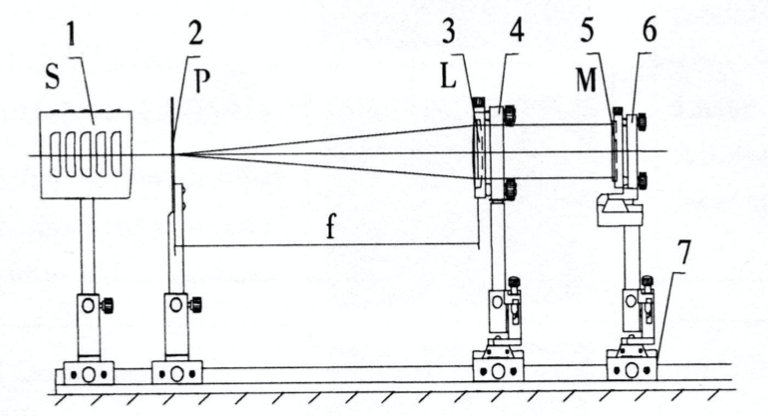
\includegraphics[width=0.8\linewidth]{scheme_1}
	\caption{Схема расположения оптических элементов в опыте по определению фокусного расстояния линзы с использованием плоского зеркала. На рисунке изображены следующие элементы: 1~-- осветитель S; 2~-- объект P (LMP-141); 3~-- собирающая линза L ($f=150$ мм); 4, 6~-- двухосевой держатель оптических элементов (LMP-07); 5~-- плоское зеркало М}
	\label{fig:1_1}
\end{figure}

\subsection{Определение фокусного расстояния с помощью экрана}

Этот способ основывается на том, что в случае, когда расстояние от предмета до экрана превышает $4F$, появляется два положения линзы, в которых получается четкое изображение предмета на экране. Схема опыта представлена на рисунке \ref{fig:1_2}

Пусть $d$ --- расстояние от предмета до линзы, $f$ --- расстояние от линзы до изображения, $L$ --- расстояние между линзой и изображением (экраном). В таком случае, в силу обратимости лучей, становится понятно, что $d_1 = f_2$, и $d_2 = f_1$. Пусть необходимая сдвижка для получения второго изображения равна $l$. Тогда:

\begin{align*}
	d_1 &= \frac{L - l}{2} \\
	d_2 &= \frac{L + l}{2}
\end{align*}

С учетом формулы тонкой линзы, получим:

\begin{equation}
	F = \frac{L^2 - l^2}{4L}
\end{equation}

Таким образом, необходимо определить необходимую сдвижку линзы $l$ из первого положения, в котором появляется четкое изображение предмета, до второго при заданном $L$. Для верности данное действие было проделано трижды для различных $L$, а в каждой серии экспериментов линзу переворачивали другой стороной и вновь измеряли $l$.

В ходе трех серий экспериментов были получены следующие результаты:

\begin{center}
	\begin{tabular}{|c|c|c|c|}
		\hline
		№ серии & $L$, мм & $l_1$, мм & $l_2$, мм \\
		\hline
		1 & $790 \pm 0.5$ & $397 \pm 0.5$ & $400 \pm 0.5$ \\
		\hline
		2 & $935 \pm 0.5$ & $570 \pm 0.5$ & $563 \pm 0.5$ \\
		\hline
		3 & $983 \pm 0.5$ & $615 \pm 0.5$ & $610 \pm 0.5$ \\
		\hline
	\end{tabular}
\end{center}

После усреднения всех полученных фокусных расстояний, получаем: % Посчитать погрешность и как следствие число знаков

\begin{equation*}
	\boxed{
		F = 148.507 \pm 0.5 \text{ мм}}
\end{equation*}

\begin{figure}[H]
	\centering
	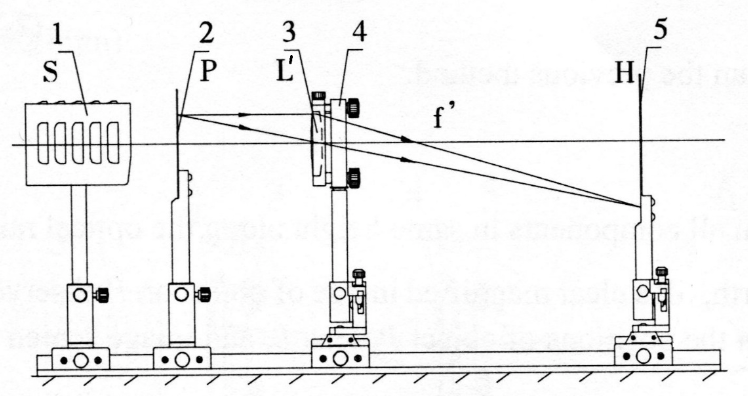
\includegraphics[width=0.7\linewidth]{scheme_2}
	\caption{Схема расположения оптических элементов в опыте по определению фокусного расстояния линзы с использованием экрана. На рисунке изображены следующие элементы: 1~-- осветитель S; 2~-- объект P (LMP-14); 3~-- собирающая линза L' ($f=150$ мм); 4~-- двухосевой держатель оптических элементов (LMP-07); 5 – экран Н}
	\label{fig:1_2}
\end{figure}

\section{Определение фокусного расстояние оптической системы с помощью метода Аббе}

Фокусное расстояние оптической системы может быть измерено также с помощью метода Аббе. Получим расчетную формулу:

Предположим, что линейный размер предмета равен $y$, а находится он на расстоянии $x_1$ от главного фокуса $F$ \textbf{положительной} оптической системы. Изображение предмета в таком случае имеет размер $y_1$, а линейное увеличение равно $\beta_1 = y_1 / y = F / x$. Если же теперь передвинуть предмет на небольшое расстояние $\Delta x$, то увеличение изменится и станет равным $\beta_2 = y_2 / y = F / x$. В таком случае, легко получить:

\begin{equation}
	F = \frac{\Delta x}{\frac{1}{\beta_1} - \frac{1}{\beta_2}}
	\label{eq:abbe}
\end{equation}

Таким образом, необходимо определить линейное увеличение $\beta_1$ в одном положении линзы, и линейное увеличение $\beta_2$ в сдвинутом относительно первого на $\Delta x$. Схема опыта представлена на рисунке \ref{fig:2}.

В результате экспериментов были полученные следующие данные:

\begin{center}
	\begin{tabular}{|c|c|c|}
		\hline
		$\beta_1$ & $\Delta x$, мм & $\beta_2$ \\
		\hline
		1 & 10 & 1.5 \\
		\hline
	\end{tabular}
\end{center}

Тогда, с учетом формулы (\ref{eq:abbe}), получаем значение фокусного расстояния:

\begin{equation*} % Погрешность
	\boxed{
	F = 30 \text{мм}}
\end{equation*}

\begin{figure}[H]
	\centering
	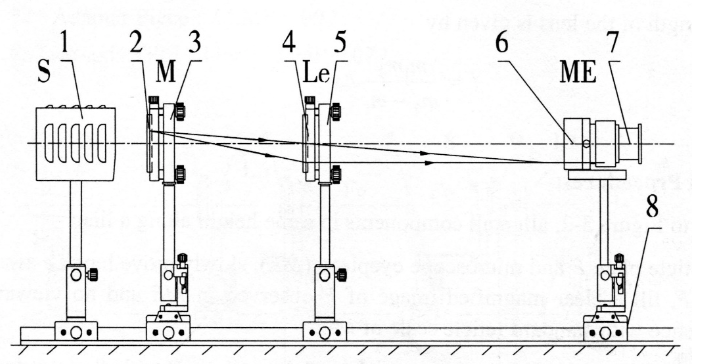
\includegraphics[width=0.7\linewidth]{scheme_3}
	\caption{Схема расположения оптических элементов в опыте по определению фокусного расстояния линзы с помощью метода Аббе. На рисунке изображены следующие элементы: 1~-- осветитель S; 2~-- слайд с делениями M (Reticle); 3~-- держатель бипризм (LMP-41); 4~-- линза Le ($f=35$ мм); 5~-- двухосевой держатель оптических элементов (LMP-07); 6~-- окуляр микроскопа МЕ; 7~-- держатель микроскопа (LMP-09)}
	\label{fig:2}
\end{figure}

\section{Определение фокусное расстояние и положение главных плоскостей системы линз}

Пусть у нас теперь есть оптическая система, которая состоит из двух центрированных собирающих линз, которые расположены на известном расстоянии друг от друга. 

Известным является факт, что если система состоит из двух собирающих линз, то фокусное расстояние системы можно рассчитать следующим образом:

\begin{equation}
	\frac{1}{F} = \frac{1}{F_1} + \frac{1}{F_2} - \frac{l_{12}}{F_1 F_2}
	\label{eq:double_lens}
\end{equation}

Здесь $l_{12}$ --- расстояние между линзами.

Сперва определим фокусное расстояние с помощью метода Аббе. Схема опыта представлена на рисунке \ref{fig:3_1}. После эксперимента были получены следующие данные:

\begin{center}
	\begin{tabular}{|c|c|c|}
		\hline
		$\beta_1$ & $\Delta x$, мм & $\beta_2$ \\
		\hline
		1.6 & 30 & 1.2 \\
		\hline
	\end{tabular}
\end{center}

Тогда по формуле (\ref{eq:abbe}) получаем:

\begin{equation*}
	\boxed{F_{abbe} = 150 \text{ мм}}
\end{equation*}

Поскольку фокусные расстояния каждой из линз известны (написаны на их ободе) и равны $F_1 = 190 \text{ мм}$ и $F_2 = 300 \text{ мм}$, по формуле же (\ref{eq:double_lens}), которая выведена для конкретной системы, получим:

\begin{equation*}
	\boxed{F_{theor} = 144 \text{ мм}}
\end{equation*}

Для определения фокальных плоскостей предлагается воспользоваться еще одной линзой, которая была установлена перед исследуемой системой на фокусном расстоянии от объекта. Таким образом, изображение от нее оказывается на бесконечности и, следовательно, проходя через оптическую систему оказывается в задней фокальной плоскости, что позволяет нам определить ее положение. В ходе эксперимента было определено взаимное положение фокальных плоскостей относительно оптической системы, представленное на рисунке \ref{fig:3_2}.

\begin{figure}[H]
	\centering
	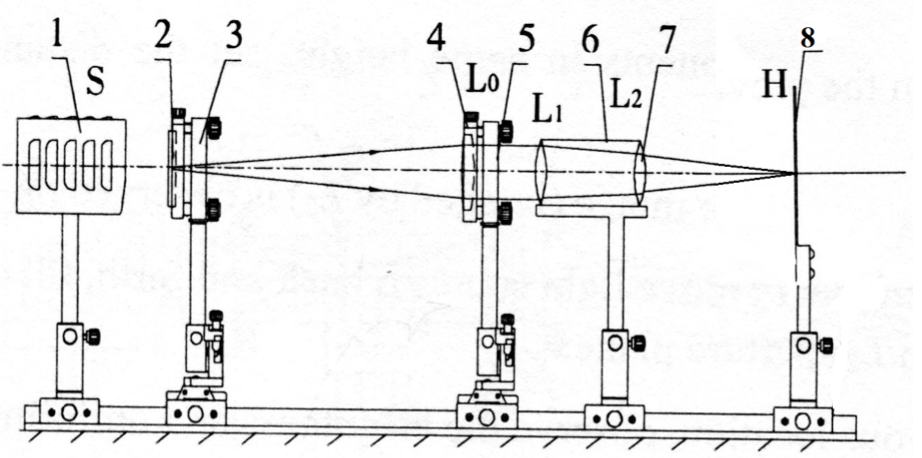
\includegraphics[width=0.7\linewidth]{scheme_4}
	\caption{Схема расположения оптических элементов в опыте по определению фокусного расстояния оптической системы с помощью метода Аббе. На рисунке изображены следующие элементы: 1~-- осветитель S; 2~-- слайд с линейкой (Millimetre Ruler); 3~-- держатель бипризм (LMP-41); 4~-- линза L0 ($f=150$ мм); 5~-- двухосевой держатель оптических элементов (LMP-07); 6~-- оптическая система, состоящая из линз L1 ($f=190$ мм) и L2 ($f=300$~мм); 7~-- держатель группы линз (LMP-28); 8~-- экран Н (LMP-13)}
	\label{fig:3_1}
\end{figure}

\begin{figure}[H]
	\centering
	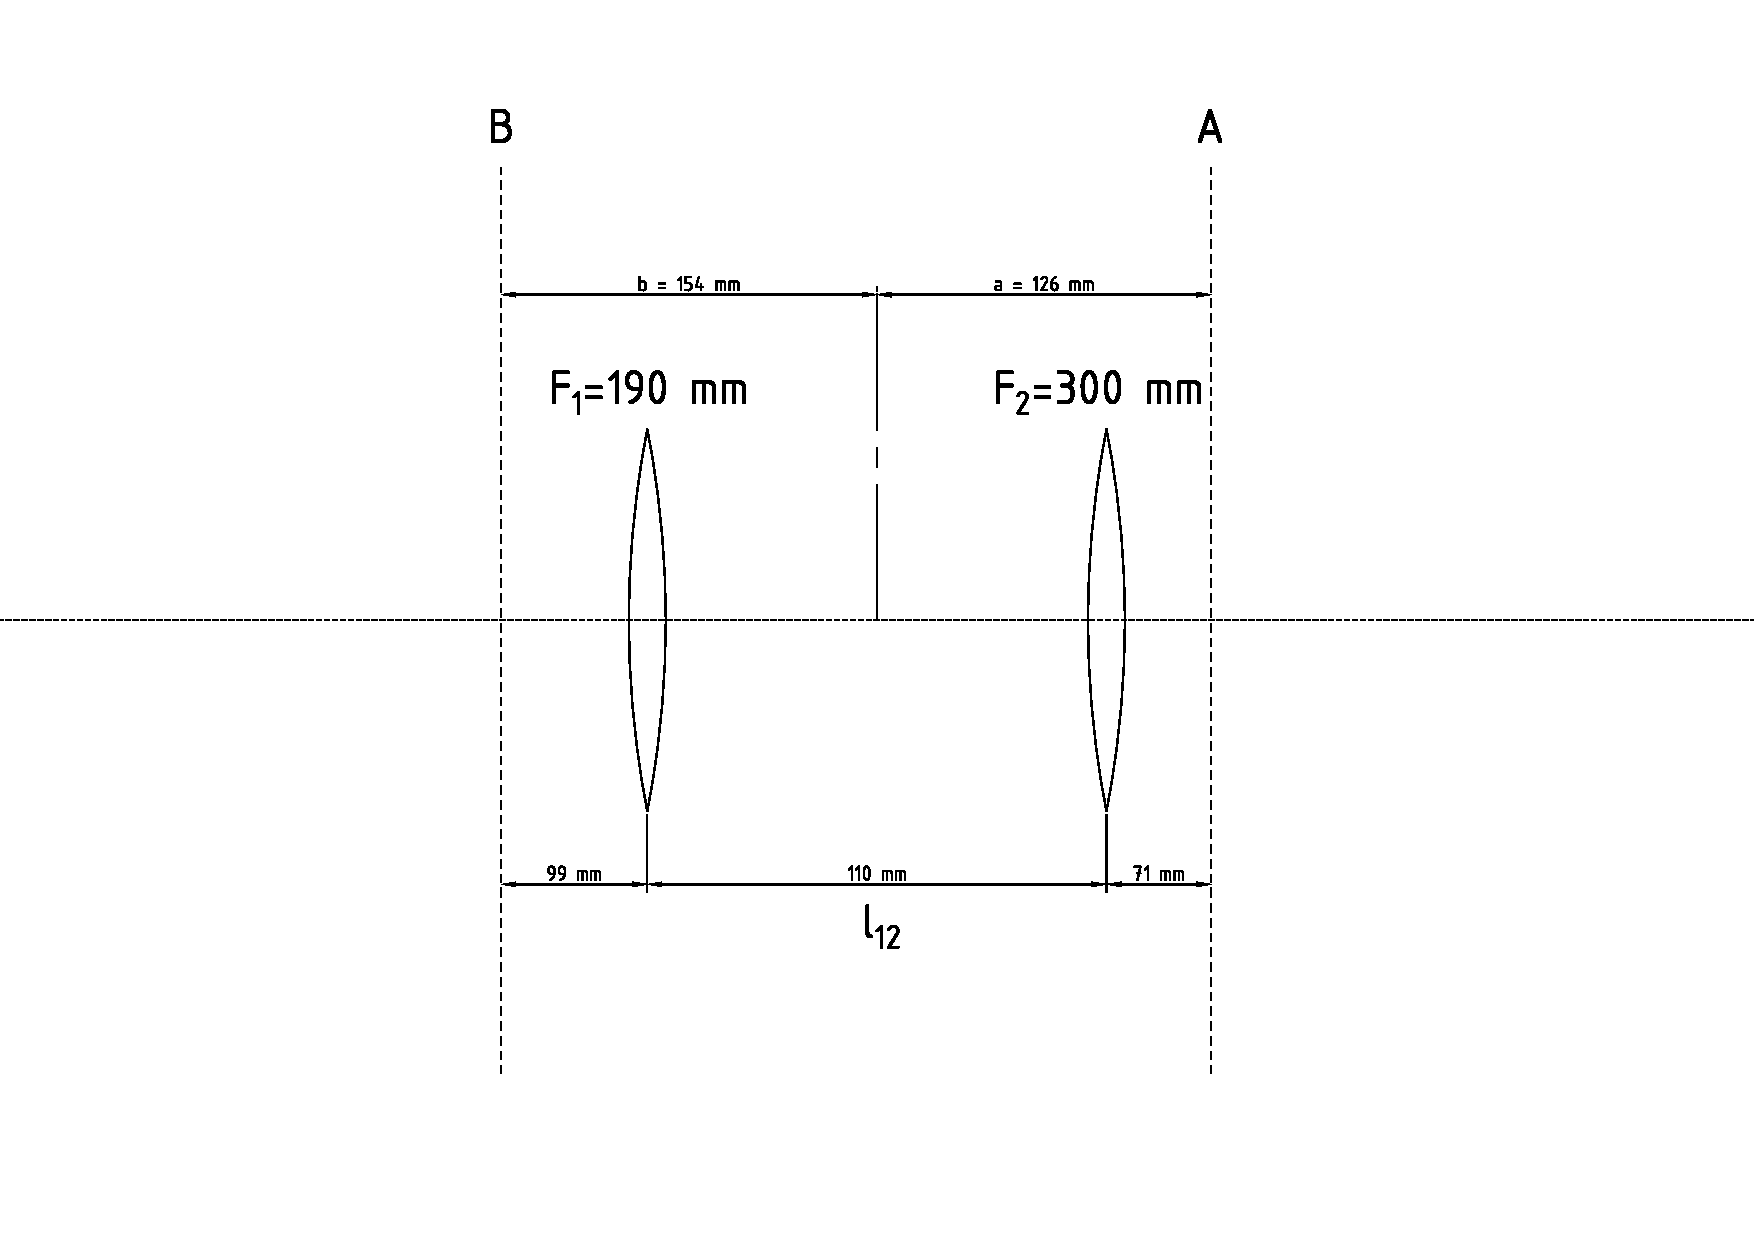
\includegraphics[width=\linewidth]{lenses}
	\caption{Взаимное расположение фокальных плоскостей оптической системы относительно линз}
	\label{fig:3_2}
\end{figure}


\section{Определение углового увеличения телескопа}

Для определения углового увеличения телескопа было сделано следующее.

После слайда-линейки, который выступает в роли объекта, была установлена на ее фокусном расстоянии линза. Это позволяет получить параллельный пучок света, с которым обычно и работают при использовании телескопа. После этого с помощью зрительной трубы было определено число штрихов на линейке $N_1 = 10$, которые укладывались в поле зрения трубы. Затем после линзы была установлена собранная труба Кеплера ($F_1 = 190 \text{ мм, } F_2 = 105 \text{ мм}$) и данная операция была проделана еще раз, с получившимся $N_2 = 5$.

Угловым увеличением в таком случае по определению будет являться:

\begin{equation}
	\boxed{
	\gamma_N = \frac{N_1}{N_2} = 2}
\end{equation}

С другой стороны, воспользовавшись законами геометрии, возможно получить еще одно соотношение:

\begin{equation*}
	\gamma_f = \frac{F_1}{F_2} = 1.81
\end{equation*}

Как видно, полученные двумя различными способами значения совпадают с известной точностью.

\section{Вывод}

\begin{enumerate}
	\item Ознакомление с приборами и методами определения фокуса было проведено.
	
	\item Было установлено фокусное расстояние линзы с помощью двух методов: с использованием зеркала и с использованием экрана, которые дали результаты, неплохо сходящиеся с реальностью и друг с другом: $F = 151\pm 0.5$~мм для метода с зеркалом и $F = 148.507 \pm 0.5$~мм для метода с использованием экрана. %Погрешности для экрана и число знаков
	
	\item С помощью метода Аббе было установлено фокусное расстояние линзы $F = 30$~мм. %Погрешность
	
	\item  Для имеющейся системы из двух собирающих линз было определено ее фокусное расстояние, оказавшееся равным $F_{abbe} = 150 \text{ мм}$ по данным эксперимента и $F_{theor} = 144 \text{ мм}$ по предсказаниям теории. Было также получено расположение главных плоскостей системы относительное ее центра, представленное на рисунке \ref{fig:3_2}. %погрешности.
	
	\item Было определено угловое увеличение телескопа, которое оказалось равным $\gamma_N = 2$ из эксперимента и $\gamma_f = 1.81$ из теории. 
\end{enumerate}





\end{document}